\documentclass[a4paper,12pt]{article}
\usepackage[hmargin=2.5cm,vmargin=2.5cm]{geometry}

\usepackage[utf8]{inputenc}   % le fichier .tex est en UTF-8     
\usepackage[francais]{babel}  %typo française                    
\usepackage[T1]{fontenc}      % encodage des fonts latex         
\usepackage{lmodern}                                             
\usepackage{microtype}        % typo supplémentaires             



\usepackage{graphicx} %inclusion de graphiques


\usepackage{hyperref} % liens dans le pdf
\hypersetup{%
  pdftitle={Title},
  pdfauthor={Author1, Author2},
  pdfkeywords={keywords}
  pdfsubject={article},
  colorlinks=true,
  linkcolor=black,
  urlcolor=black,
  citecolor=black
}


\title{1CKA, structure repliée contre structure dépliée} % c'est la déclaration



\begin{document}

\maketitle % c’est ici que le titre est inséré


    Trois heuristiques ont été utilisées:\\
    L'heuristique "somme et différence" où l'optimisation est faite avec un test sur la somme des énergies des deux structures et un test sur la différence structure repliée moins structure dépliée.\\ 
    L'heuristique "seuil et différence" contient un seuil sur la somme (à la valeur de -110) et un test sur la différence structure repliée moins structure dépliée.\\
    L'heuristique "somme" contient seulement la somme des énergies des deux structures.\\

    Pour chaque heuristique, 100000 séquences de rotamères ont été générées par proteus version 28.3.
    Les énergies de références utilisées: GBE4SA. pour la structure dépliée et "optref" pour la structure repliée. 
        
    
  \begin{sffamily}

    \section{L'heuristique "somme et différence"}
 
    
   
   \begin{figure}[!htbp]
     \centering
     \includegraphics[width=18cm]{heur2_sort1_seqlogo.eps}
     \begin{bfseries}
      \resizebox{18cm}{3mm} {
        \begin{tabular}{*{57}{c}}
          3.9 & 4.3 & 3.4 & 2.9 & 2.1 & 2.1 & 4.0 & 1.9 & 3.1 & 2.4 & 3.9 & 1.0 & 3.4 & 4.1 & 3.6 & 4.3 & 2.9 & 1.3 & 1.0 & 3.2 & 4.8 & 3.9 & 1.0 & 2.0 & 2.6 & 2.2 & 4.6 & 1.9 & 3.1 & 2.7 & 2.8 & 1.0 & 2.9 & 3.1 & 3.3 & 1.9 & 3.5 & 1.8 & 1.8 & 2.8 & 2.7 & 3.2 & 4.1 & 1.0 & 4.2 & 3.7 & 1.0 & 2.9 & 1.6 & 1.0 & 3.7 & 1.0 & 1.8 & 1.9 & 4.4 & 4.5 & 2.8 \\
      \end{tabular}
      }
     \end{bfseries}
     \caption{Séquence logo et exponentiel de l'entropie par position, pour les 10000 premières séquences après un tri sur énergie de la somme.}
     \label{heur_somme_et_diff_tri_somme}
   \end{figure}

   \begin{figure}[!htbp]
     \centering
     \includegraphics[width=18cm]{heur2_sort2_seqlogo.eps}
     \begin{bfseries}
      \resizebox{18cm}{3mm} {
        \begin{tabular}{*{57}{c}}
          3.8 & 4.7 & 3.7 & 3.4 & 2.5 & 2.2 & 4.2 & 1.9 & 3.4 & 2.8 & 3.8 & 1.0 & 3.4 & 4.4 & 3.7 & 4.4 & 3.2 & 1.4 & 1.0 & 3.5 & 4.7 & 4.1 & 1.0 & 2.4 & 3.0 & 2.4 & 4.9 & 2.4 & 3.5 & 3.1 & 3.3 & 1.0 & 3.4 & 3.2 & 3.4 & 2.4 & 3.8 & 2.3 & 2.0 & 3.5 & 3.2 & 3.6 & 4.3 & 1.0 & 4.3 & 4.1 & 1.0 & 3.3 & 2.0 & 1.0 & 4.1 & 1.0 & 1.9 & 2.3 & 4.3 & 4.3 & 3.2 \\
      \end{tabular}
      }
     \end{bfseries}
     \caption{Séquence logo et exponentiel de l'entropie par position, pour les 10000 premières séquences après un tri sur énergie de la différence.}
     \label{heur_som_et_diff_tri_diff}
   \end{figure}

   \newpage
    \section{L'heuristique "seuil et différence"}
    
   \begin{figure}[!htbp]
     \centering
     \includegraphics[width=18cm]{heur4_sort1_seqlogo.eps}
     \begin{bfseries}
      \resizebox{18cm}{3mm} {
        \begin{tabular}{*{57}{c}}
          3.9 & 4.8 & 3.5 & 3.4 & 2.4 & 2.1 & 4.1 & 2.0 & 3.5 & 2.6 & 3.9 & 1.0 & 3.5 & 4.4 & 3.7 & 4.5 & 3.0 & 1.5 & 1.0 & 3.5 & 4.9 & 4.0 & 1.0 & 2.4 & 3.2 & 2.4 & 4.9 & 2.6 & 4.0 & 3.5 & 3.0 & 1.0 & 3.9 & 3.3 & 3.6 & 2.8 & 3.5 & 2.5 & 1.8 & 3.6 & 3.0 & 3.7 & 4.4 & 1.0 & 4.3 & 4.0 & 1.0 & 3.2 & 2.0 & 1.0 & 4.2 & 1.0 & 2.2 & 2.2 & 4.4 & 4.5 & 2.9 \\
      \end{tabular}
      }
     \end{bfseries}
     \caption{Séquence logo et exponentiel de l'entropie par position, pour les 10000 premières séquences après un tri sur énergie de la somme.}
     \label{heur_somme_et_diff_tri_somme}
   \end{figure}

   \begin{figure}[!htbp]
     \centering
     \includegraphics[width=18cm]{heur4_sort2_seqlogo.eps}
     \begin{bfseries}
      \resizebox{18cm}{3mm} {
        \begin{tabular}{*{57}{c}}
          3.8 & 4.7 & 3.7 & 3.4 & 2.6 & 2.2 & 4.2 & 2.0 & 3.5 & 2.8 & 3.8 & 1.0 & 3.4 & 4.4 & 3.7 & 4.3 & 3.2 & 1.6 & 1.0 & 3.5 & 4.7 & 4.1 & 1.0 & 2.5 & 3.0 & 2.5 & 4.9 & 2.4 & 3.6 & 3.1 & 3.3 & 1.0 & 3.5 & 3.3 & 3.4 & 2.4 & 3.8 & 2.3 & 2.0 & 3.5 & 3.3 & 3.7 & 4.3 & 1.0 & 4.3 & 4.1 & 1.0 & 3.4 & 2.1 & 1.0 & 4.1 & 1.0 & 1.9 & 2.3 & 4.3 & 4.4 & 3.2 \\
      \end{tabular}
      }
     \end{bfseries}
     \caption{Séquence logo et exponentiel de l'entropie par position, pour les 10000 premières séquences après un tri sur énergie de la différence.}
     \label{heur_som_et_diff_tri_diff}
   \end{figure}
   \newpage
    \section{L'heuristique "somme "}
    
   \begin{figure}[!htbp]
     \centering
     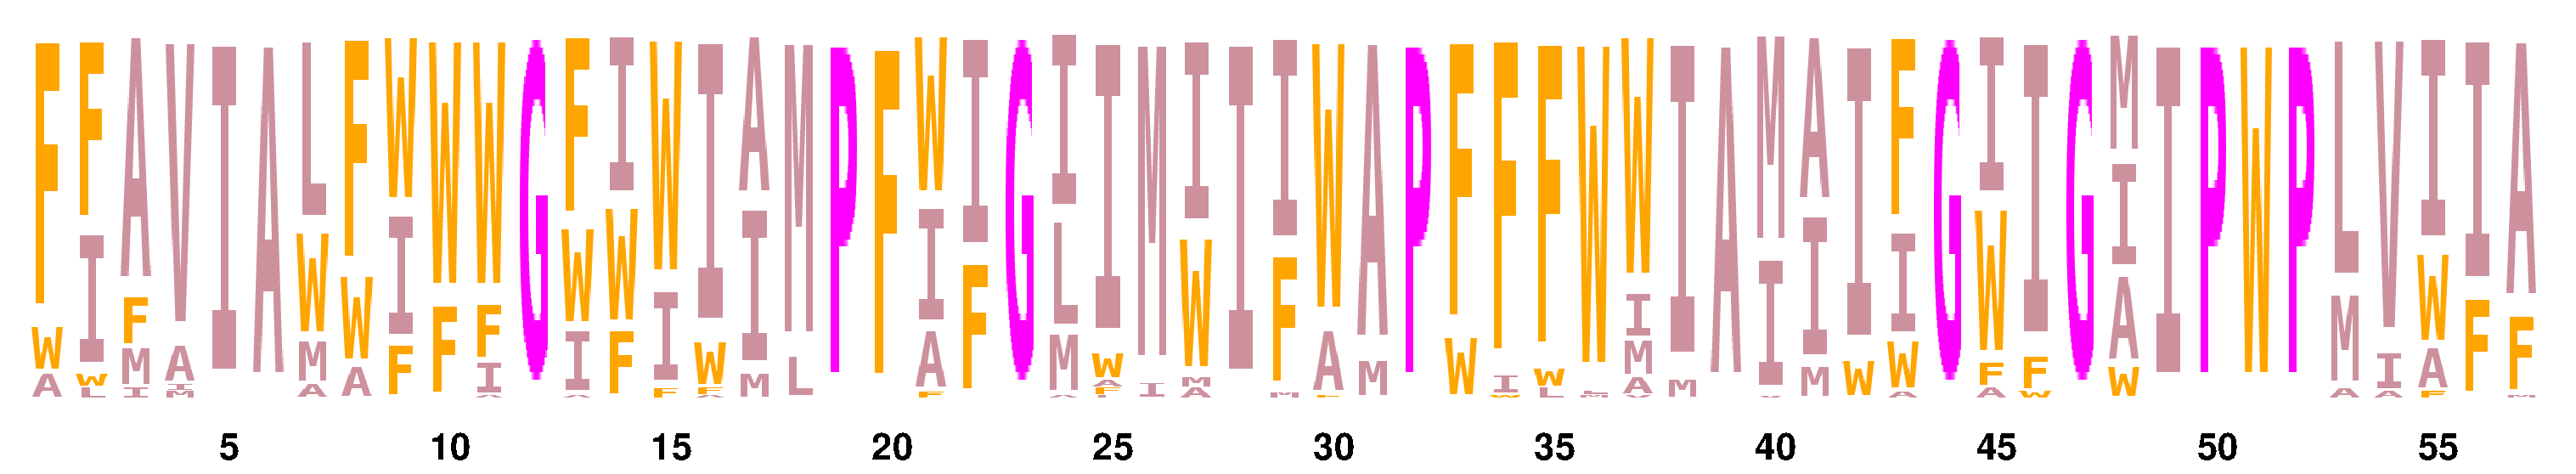
\includegraphics[width=18cm]{heur3_sort1_seqlogo.eps}
     \begin{bfseries}
      \resizebox{18cm}{3mm} {
        \begin{tabular}{*{57}{c}}
          1.3 & 2.0 & 2.2 & 1.4 & 1.1 & 1.0 & 2.2 & 1.4 & 2.0 & 1.0 & 1.4 & 1.0 & 1.7 & 2.0 & 1.8 & 1.6 & 2.0 & 1.0 & 1.0 & 1.0 & 2.8 & 2.0 & 1.0 & 1.1 & 1.6 & 1.0 & 2.2 & 1.0 & 2.0 & 1.6 & 1.4 & 1.0 & 1.0 & 1.2 & 1.2 & 1.1 & 2.0 & 1.0 & 1.0 & 1.0 & 2.0 & 1.5 & 2.0 & 1.0 & 2.2 & 1.4 & 1.0 & 2.3 & 1.0 & 1.0 & 1.0 & 1.0 & 1.1 & 1.1 & 2.5 & 1.8 & 1.8 \\
      \end{tabular}
      }
     \end{bfseries}
     \caption{Séquence logo et exponentiel de l'entropie par position, pour les 10000 premières séquences après un tri sur énergie de la somme.}
     \label{heur_somme_et_diff_tri_somme}
   \end{figure}

   \begin{figure}[!htbp]
     \centering
     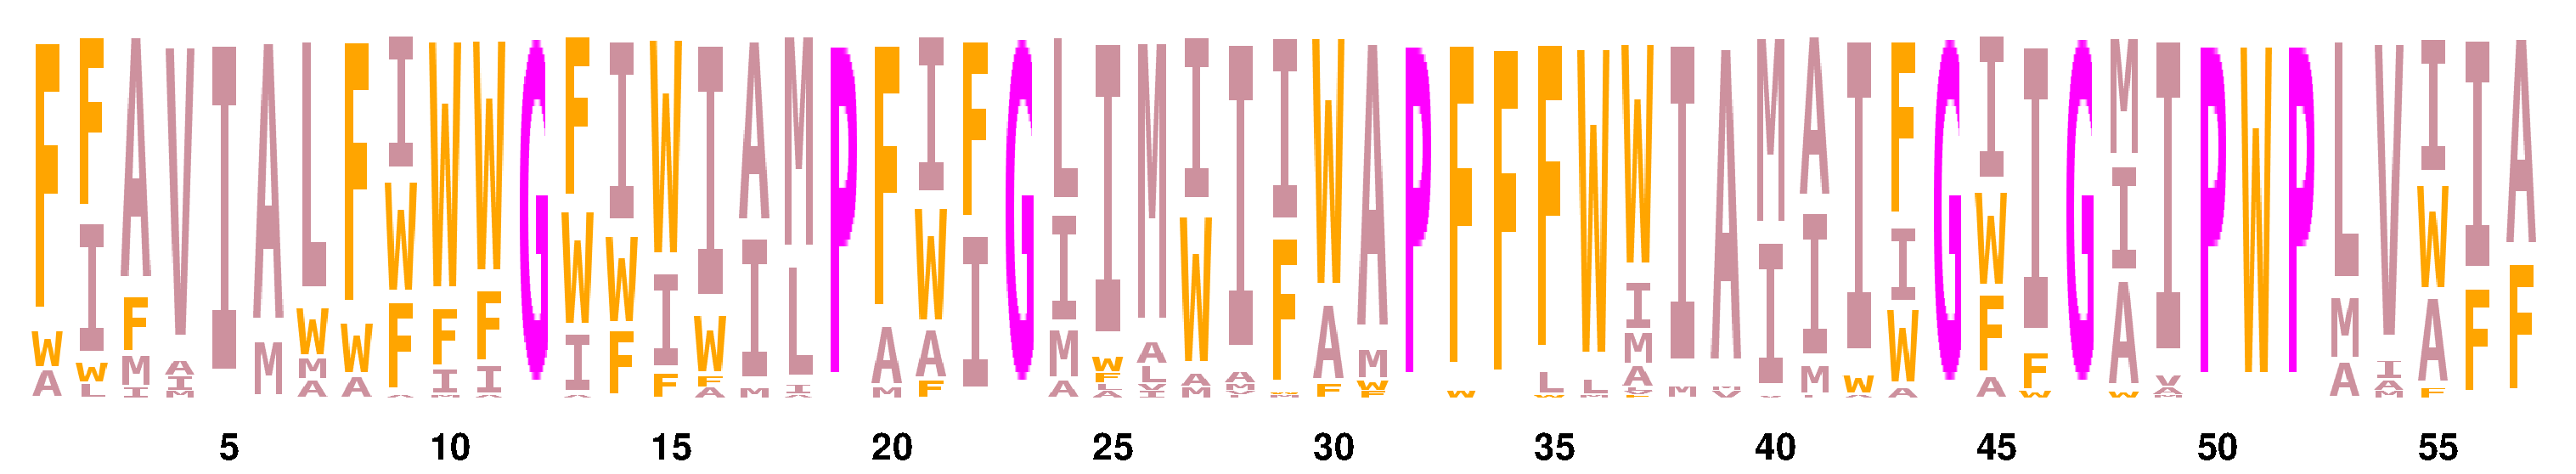
\includegraphics[width=18cm]{heur3_sort2_seqlogo.eps}
     \begin{bfseries}
      \resizebox{18cm}{3mm} {
        \begin{tabular}{*{57}{c}}
          1.3 & 2.0 & 2.2 & 1.3 & 1.0 & 1.6 & 1.8 & 1.3 & 2.1 & 1.3 & 1.4 & 1.0 & 1.7 & 2.0 & 1.8 & 1.9 & 2.0 & 1.0 & 1.0 & 1.8 & 2.7 & 2.0 & 1.0 & 1.2 & 1.4 & 1.3 & 2.3 & 1.2 & 2.0 & 1.7 & 1.6 & 1.0 & 1.0 & 1.1 & 1.3 & 1.3 & 2.2 & 1.0 & 1.2 & 1.0 & 2.0 & 1.3 & 1.9 & 1.0 & 2.4 & 1.5 & 1.0 & 2.1 & 1.1 & 1.0 & 1.0 & 1.0 & 1.4 & 1.2 & 2.9 & 1.9 & 2.0 \\
      \end{tabular}
      }
     \end{bfseries}
     \caption{Séquence logo et exponentiel de l'entropie par position, pour les 10000 premières séquences après un tri sur énergie de la différence.}
     \label{heur_somme_et_diff_tri_somme}
   \end{figure}


\section{Moyennes et écarts-types des énergies}



Pour chaque heuristique, les séquences de rotamères générées sont triées de deux façons différentes:\\
- un tri sur la somme des énergies des deux groupes pliés et déplié.\\
- un tri sur la différence d'énergie des deux groupes.
 

    \begin{table}[!htbp]
      \centering
      \resizebox{18cm}{!} {
      \begin{tabular}{|c|c|c|c||c|c||c|c|}
        \hline
        \multicolumn{2}{|c|}{} &\multicolumn{2}{c||}{Somme et différence} & \multicolumn{2}{c||}{Seuil et différence} & \multicolumn{2}{c|}{Somme} \\ \hline

   \multicolumn{2}{|c|}{Energies} & tri somme & tri différence & tri somme & tri différence & tri somme & tri différence  \\ \hline    
              &  max       &  70    &    -77         &   -105   &    -117         &  170       & 170             \\ \cline{2-8}         
   somme      & moyenne    & -67    &    -165        &   -117   &    -204         &  161       & 157             \\ \cline{2-8}      
              & écart type &  28    &    28          &    9     &     36          &   2        &  5              \\ \hline 
              & max        &  617   &    670         &    647   &     732         &   328      & 328             \\ \cline{2-8}         
   différence & moyenne    &  533   &    628         &    570   &     665         &   299      & 305             \\ \cline{2-8}      
              & écart type &  31    &    21          &    25    &     29          &    9       & 5               \\ \cline{2-8} 



        \hline
      \end{tabular}
    }
      \caption{Moyennes et écarts-types calculés pour les 20000 premières séquences après tri.}      

      \label{tab_MCvsHeur}
    \end{table}


  \end{sffamily}
\end{document}
